% Chapter 1

\chapter{Wearable devices and new human-machine interfaces: an overview}

\lhead{Chapter 1. \emph{Wearable devices and new human-machine interfaces}} % This is for the header on each page - perhaps a shortened title

%----------------------------------------------------------------------------------------

\section{Where to wear an extra eye?}
Positioning an optical device on the human body is quite a problematic task, as occlusion, motion, social issues as well as criteria related to the purpose of the device must be taken into account.\footnote{\url{http://www.robots.ox.ac.uk/~wmayol/3D/nancy_matlab.html}}. Following the work of Mayol \etal \cite{mayol2001positioning}, in this section we give a detailed overview on the best places where to put a wearable camera.

Cameras used for wearable applications fall into two categories for this discussion; static narrow-view devices and omnidirectional devices. Omnidirectional devices include catadioptric, fish-eye and active systems where either the entire field-of-viewis imaged at low resolution, or in the active case the high-resolution narrow-view sensor moved to any orientation. Narrow-view static cameras can only ever see a small part of the user or their environment, and placement is therefore entirely driven by the task. For wide-angle or omnidirectional sensors placement is less constrained and a range of positions are possible. 
\begin{figure}[htbp]
	\centering
		\includegraphics[page=3]{Figures/mayol_etal_ouel224101_cropped.pdf}
	\caption[An Electron]{An electron (artist's impression).}
	\label{fig:Electron}
\end{figure}

\begin{figure}[htbp]
	\centering
		\includegraphics[page=4]{Figures/mayol_etal_ouel224101_cropped.pdf}
	\caption[An Electron]{An electron (artist's impression).}
	\label{fig:Electron}
\end{figure}

\begin{figure}[htbp]
	\centering
		\includegraphics[page=5]{Figures/mayol_etal_ouel224101_cropped.pdf}
	\caption[An Electron]{An electron (artist's impression).}
	\label{fig:Electron}
\end{figure}

%----------------------------------------------------------------------------------------

\section{3D cameras}


%----------------------------------------------------------------------------------------

\section{In Closing}
